% Template for ICIP-2019 paper; to be used with:
%          spconf.sty  - ICASSP/ICIP LaTeX style file, and
%          IEEEbib.bst - IEEE bibliography style file.
% --------------------------------------------------------------------------
\documentclass{article}
\usepackage{spconf,amsmath,graphicx,booktabs}

% Example definitions.
% --------------------
\def\x{{\mathbf x}}
\def\L{{\cal L}}

% Title.
% ------
\title{APPLYING MACHINE LEARNING REGRESSION AND CLASSIFICATION TO PREDICT RELAPSE FREE SURVIVAL AND PATHOLOGICAL COMPLETE RESPONSE FOR BREAST CANCER PATIENTS}
%
% Single address.
% ---------------
\name{Ayush Ranjan (20601369), Amit Kumar (20594315), Rohan Sood (20600751), Dominic Mwita (20442271)\thanks{}}
\address{University of Nottingham}
%
% For example:
% ------------
\address{School of Computer Science University of Nottingham\\
	Computer Science\\
	Nottingham}
%
% Two addresses (uncomment and modify for two-address case).
% ----------------------------------------------------------
%\twoauthors
%  {A. Author-one, B. Author-two\sthanks{Thanks to XYZ agency for funding.}}
%	{School A-B\\
%	Department A-B\\
%	Address A-B}
%  {C. Author-three, D. Author-four\sthanks{The fourth author performed the work
%	while at ...}}
%	{School C-D\\
%	Department C-D\\
%	Address C-D}
%
\begin{document}
%\ninept
%
\maketitle
%
\begin{abstract}
	Different regression and classification models were trained to predict relapse free survival (RFS) and pathological complete response (PCR), respectively to find the best model for each task. The paper used breast cancer patients dataset from  The American College of Radiology Imaging Network (I-SPY 2 TRIAL). To predict RFS of patients XGBoost model delivered the best results compared with random forest, support vector machines. Classification problem is the case of imbalanced classes where the class of interest, patients that achieved PCR is the minority class. Thus, the interest was to achieve high balanced classification accuracy. En ensemble of voting classifiers consisting logistic regression, random forest and XGboost outperformed individual models by achieving 61.4 percent balanced accuracy, albeit at the cost of slightly higher variance. More data or relevant features may be necessary for the trained models to achieve better prediction outcomes. 
\end{abstract}
%
\begin{keywords}
	Imbalanced classes, logistic regression, random forest, support vector machines, XGBoost, balanced accuracy score
\end{keywords}
%
\section{INTRODUCTION}
\label{sec:intro}
This paper applies supervised machine learning algorithms on breast cancer patients public dataset extracted from The American College of Radiology Imaging Network to predict pathological complete response - PCR (classification) and relapse free survival - RFS of the patients for stratification before provision chemotherapy treatment. The aim is to build different machine learning models and select the best one for the task given nature of dataset. 

Similar studies have been conducted, applying different methods with varying performance in prediction based on selected metrics. Regression models such as General Linear Regression, Gradient Boosted Machines (GBM) and Random Forests were applied in  \cite{bartholomai2018lung} to predict survival time for lung cancer patients in months using data from Surveillance, Epidemiology, and End 
Results (SEER). The methods achieved varying performances in different conditions, for instance length of survival time--implying that no best model for every task--the choice and performance of an algorithm depends on many factors and specifics of the problem itself.

The classification task aimed at predicting PCR status is a binary in nature  because the target has two outcomes--achieved PCR (positive outcome) or not. The dataset contains imbalanced classes with respect to target variable PCR where it contains around 22 percent of positive samples, the rest are negative samples. This makes prediction accuracy misleading because the model can do a good job in predicting the majority classes but poorly on minority class because the model tends to  over-fit majority class \cite{spelmen2018review,pristyanto2018}. Imbalanced or skewed data is among biggest challenges in machine learning classification in real-world scenario as most of data is imbalanced and the cases of interest is from minority class. Various workarounds have been proposed in literature to enhance model prediction. As in \cite{spelmen2018review,sukhanov2015}, these include sampling based approaches  of oversampling minority classes, undersampling majority class, cost sensitive-learning and generating synthetic samples for minority class known as Synthetic Minority-Oversampling Technique (SMOTE). This study adopts cost-sensitive learning which works by assigning higher weight on misclassification errors for instances belonging to the minority class.  



\section{METHODS}
\label{sec:methods}
\subsection{Data Preprocessing}
The dataset used contains 400 instances in with 5 missing cases in the target variable--PCR for classification, these were then dropped to minimize the risk of misleading results by imputing them. Before further processing, 20 percent of instances in dataset was reserved for testing to the so called avoid data snooping bias which provide a semblance of good performance because data from the test set leaked \cite{geron2022hands}. Train-test split was stratified to ensure that the training set contains positive instances in the same proportion as in the original dataset. For regression task--predicting Relapse Free Survival (RFS), all 400 cases were preserved as no missing values were present in target variable.The missing cases for features were imputed using k-nearest neighbour method. Different approaches were used to transform features depending on the model being trained. 

Both feature selection and dimensionality reduction methods were applied to avoid the curse of dimensionality where by data points are sparse in the feature space leading to over-fitting \cite{geron2022hands}. ANOVA test was used to select categorical features for regression task while for continuous features (extracted from image), Principal Components Analysis (PCA) was applied. Nevertheless, correlation between continuous features and target RFS was very weak suggesting non-linear relationship. 
To handle outliers--which were numerous in image-based data--two methods were applied: robust scaler and replacement of feature values with median for values falling above or below 3 times the interquartile range. The robust scaler from sklearn library works by substracting the median from data and dividing by interquartile range. These approaches were used depending the model being trained. 

\subsection{Models}
To predict RFS three non-linear methods were applied, namely Random Forest (RF), Support Vector Machines (SVM) and XGBoost regressor. Their performance was evaluated using mean absolute error (MSE). For PCR classification RF, SVM, Logistic Regression and XGBoost were trained with cost-sensitive learning methods to handle imbalanced classes. SMOTE was attempted but resulted in models with high variance, hence dropped. Cost-sensitive learning was chosen because it handles misclassification better than minority oversampling which is prone to overfitting and majority  undersampling which leads to information loss \cite{abokadr2023imbalanced}. \\

\noindent\textit{Random Forest}\\
Random forests algorithm is an ensemble of decision trees which grows numerous decision trees using different subsets of features and training examples, and the final prediction is obtained by aggregating predictions from individual decision trees. This makes random forests are amongst the most powerful machine learning algorithms can decipher complex non linear patterns which makes them prone to overfitting. Random forests have inbuilt feature selection and can handle large datasets \cite{geron2022hands}. 

For predicting RFS two random forests models were trained, one with scaled data and the other without scaled data. Model hyperparameters that were optimized by grid search cross-validation. The best estimator for tree built with scaled data was with 200 trees, maximum number of features of 6, and bootstrapped samples. For the one with unscaled data, optimal results were 100 trees, 10 maximum features with bootstrap sampling applied.

In classifying whether patients achieved PCR, a cost-sensitive balanced random forest with bootstrapping applied was built where by errors on misclassification of positive samples (PCR=1) are more penalized to improve model classification on minority class. Feature selection was applied to reduce dimensionality of data despite the fact that random forests have inbuilt feature selection. Three Categorical features were selected by chi-square test and  5 percent significance level. Continuous features were chosen by ANOVA test (equivalent to t-test on binary data) where 10 out of 108 features were chosen. Parameters of the model were optimized using cross validation and grid search. The best model was with 100 trees, maximum tree depth of 2, and maximum number of features of 8. \\

\noindent\textit{Support Vector Machines}\\
Support Vector Machines for regression works by ensuring most of the instances fall within the hyperplane while minimizing errors for those lying outside the plane. Given a continuous target variable $y$ and feature matrix $x$, SVM regression finds weights $w$ and biases $b$ that optimizes:

\begin{equation}
	\label{eq:svm}
	\text{min}\hspace{1pt}  \frac{1}{2}||w||^{2} +C\sum_{i=1}^{n}\zeta_i
\end{equation}
Subjet to 
\begin{equation*}
	|y_i - (w^{T}x + b)|< \epsilon + \zeta_i
\end{equation*}

Where $C$ is a regularization hyperparameter that controls the width of the hyperplane and $\zeta$ is a slack term that represents instances outside the hyperplane. The increasing $C$ means tolerating more errors and reducing the hyperplane width. SVM is a very powerful algorithm that can perform complex non-linear regression and classification tasks but it is computationally expensive, thus suited for small and medium sized datasets.

Non-linear Support Vector Machines (SVM) was trained because exploratory data analysis did not support linear models as evidenced by weak correlation between features and Relapse Free Survival (RFS)--the target variable--the highest correlation coefficient was less than 0.25 in absolute value. LASSO with small penalty turned all feature coefficients to zero. Thus, dimensionality reduction using PCA was performed on 107 continuous features extracted from image data and retain 2 components which captures 99 percent of their variance. Based on ANOVA test categorical features were also not found to be good predictors for RFS with insignificant p-values at 5 percent level. Hyperparameter tuning by grid search suggested the best model with 'rbf' kernel, regularization parameter C=1, and margin of error tolerance (epsilon) of 0.2.

SVM trained for PCR classification with cost sensitive-learning and SMOTE had high variance hence dropped.\\


\noindent\textit{XGBoost}\\
XGboost is one of most powerful algorithm in machine learning that is computationally efficient and provide best prediction performance. It is an ensemble tree-based algorithm that works by sequentially adding trees to minimize errors made by previous tree. The trees individually are weak predictors but combined together are very powerful predictors. The subsequent trees instead of predicting target are fitted to errors made by predecessor and the final prediction is obtained by summing prediction of all trees in an ensemble \cite{Chen_2016}. The algorithm works by fitting ensemble of $k$ trees using $n$ instances and $x_i$ features by minimizing the loss function in equation \ref{eq:xgb}. 


\begin{equation}
	\label{eq:xgb}
	L^t = \sum_{i=1}^{n}l(\hat{y_i}^{t-1},y_i)+f_t(x_i))+\Omega(f_k)
\end{equation}
Where $\hat{y_i}^t$ is prediction of example $i$ at iteration $t$, $f_t$ is a tree, $k$ is number of trees the term $\Omega$ penalizes complexity of the model to prevent overfitting. The algorithm greedily add tree $f_t$ that improves the model. Nonetheless, the algorithm is complex and has so many hyperparameters to tune to obtain the best results.

For predicting RFS, an XGBoost ensemble of 100 trees optimized by cross validation with grid search, other hyperparameters were proportion of features to build trees (0.2), learning rate (0.05), maximum tree depth (4) and regularization term for individual tree complexity - gamma (0).

XGBoost with 100 trees for classification was trained considering class imbalances by assigning higher weight to the positive class equal to the ratio of negative  to positive instances in data which was 0.78/0.22. Other model hyperparameters were optimized by cross-validation and the best model was the one with maximum fraction of features to build trees (0.15), learning rate (0.05), and maximum tree depth (3). \\

\noindent\textit{Logistic Regression}\\
Logistic regression is among widely used and simple classification algorithm that is primarily used for binary classification but can be extended to handle multi-class classification. The logistic model is expressed as:

\begin{equation}
	\label{eq:logistic}
	p_i(x) = \frac{1}{1+e^{-(wx+b)}}
\end{equation}

The function $p_i(x)$ computes the probability that a sample $i$ belongs to a positive class, RFS=1 in case of this study. The threshold used to assign samples to a positive class is usually $p_i>=0.5$ but it can be changed based on specific context of the problem of interest \cite{vemuri2020hundred}. The intrinsic parameters $w$ and $b$ are optimized by minimizing the binary cross entropy loss in Equation \ref{eq:cross-ent}. C is regularization parameter to penalize weak predictors.
\begin{equation}
	\label{eq:cross-ent}
	L = \sum_{i=1}^{n}-[y_iln(p_i)+(1-y_i)ln(1-p_i)]+C||w||
\end{equation} 
The binary logistic regression to predict PCR was fitted using cost-complexity learning to improve classification on positive samples. The model was fitted using 4 categorical features selected by chi-square test and 9 continuous features selected by ANOVA test.\\

\noindent\textit{Voting classifier ensemble}\\
Voting classifiers works by aggregating predictions from a group of classifiers (ensemble), individual classifiers may be weak learners when considered separately but together they become strong learners giving better predictive performance. This is, however, conditioned upon, independence of individual classifiers, because it allows them to make different mistakes. This paper adopts soft voting ensemble because it provides better results-- compared with hard voting ensemble--as more weight is assigned to votes with high probability \cite{geron2022hands}. An ensemble of Logistic Regression, Random Forest, and XGBoost was used to form a voting classifier.

\section{RESULTS}
\subsection{Regression}
As shown in Table \ref{tbl:reg_mae} there are small differences in mean absolute errors across trained models for both cross validation and independent test set. Nevertheless, XGBoost model produced more stable results with lowest cross validation standard deviation compared to other models. Thus XGBoost was selected among the four models presented. Noteworty, Random Forest 1 was trained with scaled data while Random Forest 2 was trained with unscaled data. 
XGBoost model produced the best results among selected models by having lowest standard deviation of cross-validation MAE.
\label{sec:results}
\begin{table}[h]
	\label{tbl:reg_mae}
	\begin{tabular}{lrrr}
\toprule
Model & Cross Validation & SD & Test \\
\midrule
Random Forest 1 & 20.124 & 2.400 & 25.199 \\
Random Forest 2 & 20.093 & 2.178 & 25.094 \\
SVM & 20.118 & 2.661 & 25.559 \\
XG boost & 20.207 & 1.967 & 25.361 \\
\bottomrule
\end{tabular}
\\
	\caption{Mean Absolute Error (MAE) for trained models}
\end{table}
 
Results obtained suggest that possibly the features used to predict RFS may not be the best for the purpose. Thus, using different features may lead to better results.

\subsection{Classification}
To predict whether breast cancer patients achieved PCR results from estimated logistic regression, random forest and XGboost vary slightly in terms of balanced accuracy score achieved. The models were also found to be relatively stable having small standard deviation of cross validation scores. The three models when combined together in an ensemble achieved the highest balanced classification accuracy for both cross-validation and test sets, however, at the cost of slightly higher variance as shown in Table \ref{tbl:clf_ba}. Therefore, a voting ensemble was chosen as the best classifier.
\begin{table}[h]
	\label{tbl:clf_ba}
	\begin{tabular}{lrrr}
\toprule
Model & Cross Validation & SD & Test \\
\midrule
Logistic & 0.615 & 0.028 & 0.593 \\
Random Forest & 0.609 & 0.070 & 0.587 \\
XGBoost & 0.610 & 0.086 & 0.591 \\
Voting Ensemble & 0.653 & 0.067 & 0.614 \\
\bottomrule
\end{tabular}
\\
	\caption{Balanced accuracy for trained models}
\end{table}

Because the models were optimized on balanced classification accuracy metric, other metrics especially precision deteriorated because balanced classification accuracy is an average of recall of both classes $PCR=1$ and $PCR=0$. Optimizing balanced classification accuracy, however reduces overall accuracy because models were trained to penalize more misclassification on minority class,  Table \ref{tbl:clf_report}.
\begin{table}[h]
	\label{tbl:clf_report}
	\begin{tabular}{lrrrr}
\toprule
 & precision & recall & f1-score & support \\
\midrule
0 & 0.84 & 0.76 & 0.80 & 62.00 \\
1 & 0.35 & 0.47 & 0.40 & 17.00 \\
accuracy & 0.70 & 0.70 & 0.70 & 0.70 \\
macro avg & 0.59 & 0.61 & 0.60 & 79.00 \\
weighted avg & 0.73 & 0.70 & 0.71 & 79.00 \\
\bottomrule
\end{tabular}
\\
	\caption{Classification report for ensemble voting classifier}
\end{table}

\section{CONCLUSION}
A dataset containing 400 patients  of which 20 percent was retained as an independent test-set was used to build machine learning models to enhance better stratification of patients before prescribing chemotherapy treatment. 
Supervised machine learning models of Random Forests, Support Vector Machines and XGBoost were trained and compared for predicting RFS for breast cancer patients. The absolute mean error for all three methods was around 20 for validation sets and higher, around 25 for a test set. XGBoost outperformed other methods considered by producing more stable results by having lowest standard deviation of cross validation MAE. The results obtained suggests that the given clinical and image-based features may not be the best for predicting RFS. With more informative features and/ or data, prediction can be improved.
For predicting patients response to initial treatment (PCR), class imbalances were considered because the dataset contained about 22 percent of patients who achieved PCR and the remaining 78 percent did not. As such, the models were trained with cost sensitive learning which penalizes more on errors. Model performance was evaluated based on balanced accuracy score which makes more sense when the distribution of classes is skewed. An ensemble of voting classifiers outperformed individual models that were aggregated by achieving highest balanced classification accuracy, but with slightly high variance. The built model may not be the best for the task, more data may be required to train better models and if more informative could be available then performance can be increased considerably.




% Below is an example of how to insert images. Delete the ``\vspace'' line,
% uncomment the preceding line ``\centerline...'' and replace ``imageX.ps''
% with a suitable PostScript file name.
% -------------------------------------------------------------------------
%\begin{figure}[htb]
%
%\begin{minipage}[b]{1.0\linewidth}
%  \centering
%  \centerline{\includegraphics[width=8.5cm]{image1}}
%%  \vspace{2.0cm}
%  \centerline{(a) Result 1}\medskip
%\end{minipage}
%%
%\begin{minipage}[b]{.48\linewidth}
%  \centering
%  \centerline{\includegraphics[width=4.0cm]{image3}}
%%  \vspace{1.5cm}
%  \centerline{(b) Results 3}\medskip
%\end{minipage}
%\hfill
%\begin{minipage}[b]{0.48\linewidth}
%  \centering
%  \centerline{\includegraphics[width=4.0cm]{image4}}
%%  \vspace{1.5cm}
%  \centerline{(c) Result 4}\medskip
%\end{minipage}
%%
%\caption{Example of placing a figure with experimental results.}
%\label{fig:res}
%%
%\end{figure}


% To start a new column (but not a new page) and help balance the last-page
% column length use \vfill\pagebreak.
% -------------------------------------------------------------------------
%\vfill
%\pagebreak




% -------------------------------------------------------------------------
\bibliographystyle{IEEEbib}
\bibliography{references}
\pagebreak
\begin{figure*}
	\caption{Contribution table}
	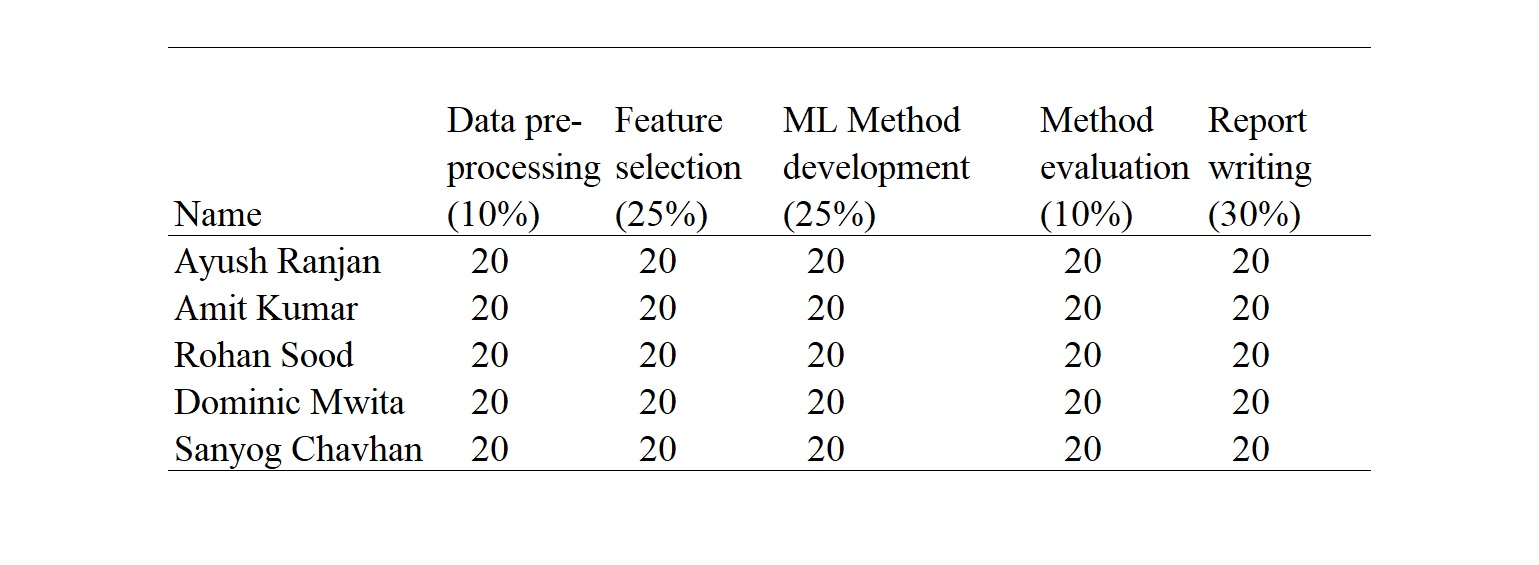
\includegraphics{contributions.jpg}
\end{figure*}

\end{document}
